% !TeX program = xelatex
% !TeX options = -shell-escape
% !TEX encoding = UTF-8

% --------------------------------------------------------------
% This is all preamble stuff that you don't have to worry about.
% Head down to where it says "Start here"
% --------------------------------------------------------------

\documentclass[12pt]{article}
\usepackage[margin=2cm]{geometry} % 頁面邊距設置
\usepackage{amsmath,amssymb,amsthm} % 數學相關套件
\usepackage{graphicx} % 圖形插入
\usepackage{booktabs} % 表格線條
\usepackage[AutoFakeBold,AutoFakeSlant]{xeCJK} % 中文支援
\usepackage{fancyhdr} % 頁首頁尾設置
\usepackage{xcolor,changepage,mdframed} % 顏色與框線相關
\usepackage{titlesec} % 標題格式
\usepackage{setspace} % 行距
\usepackage{minted} % 程式碼高亮（需安裝 Python 套件 pygments）
\usepackage{booktabs}
\usepackage{caption}
\usepackage{array}
\usepackage{ulem}
\usepackage[shortlabels]{enumitem} % 列表格式
\usepackage[colorlinks=true,linkcolor=black,urlcolor=blue,citecolor=blue]{hyperref}
% 超連結
\graphicspath{{images}}

% 字體設定 (xeCJK)
\setCJKmainfont{黑體-繁}
\setCJKmonofont{Noto Sans Mono CJK TC}

% 頁首/頁尾設定 (fancyhdr)
\pagestyle{fancy}
\fancyhead[L]{NASA Lab 13} % 可以用 \leftmark 取代
\fancyhead[R]{B13901011 吳亞倫}
\fancyfoot[C]{\thepage}
\renewcommand{\headrulewidth}{0.4pt}
\renewcommand{\footrulewidth}{0pt}
\setlength{\headheight}{15pt}

% tex-fmt: off
\newtheorem*{theorem}{Theorem}
\newenvironment{lemma}[2][Lemma]{\begin{trivlist}
\item[\hskip \labelsep {\bfseries #1}\hskip \labelsep {\bfseries #2.}]}{\end{trivlist}}
\newenvironment{exercise}[2][Exercise]{\begin{trivlist}
\item[\hskip \labelsep {\bfseries #1}\hskip \labelsep {\bfseries #2.}]}{\end{trivlist}}
\newenvironment{problem}[2][Problem]{\begin{trivlist}
\item[\hskip \labelsep {\bfseries #1}\hskip \labelsep {\bfseries #2}]}{\end{trivlist}}
\newenvironment{question}[2][Question]{\begin{trivlist}
\item[\hskip \labelsep {\bfseries #1}\hskip \labelsep {\bfseries #2.}]}{\end{trivlist}}
\newenvironment{corollary}[2][Corollary]{\begin{trivlist}
\item[\hskip \labelsep {\bfseries #1}\hskip \labelsep {\bfseries #2.}]}{\end{trivlist}}
\newenvironment{solution}{\begin{proof}[Solution]}{\end{proof}}
\newenvironment{answer}{\begin{proof}[Ans]}{\end{proof}}

% 樣式設定

\setminted{frame=lines, linenos, framesep=2mm, breaklines=true, breakanywhere=true, autogobble=true}

% 自訂框線環境
\newmdenv[
  linewidth=2pt, linecolor=gray, backgroundcolor=gray!10,
  topline=false, bottomline=false, rightline=false,
  skipabove=10pt, skipbelow=10pt, innerleftmargin=10pt,
  innerrightmargin=0pt, innertopmargin=5pt, innerbottommargin=5pt
]{myquote}

\newenvironment{mycolorbox}[1][gray]{
  \renewmdenv[
    linewidth=2pt, linecolor=#1, backgroundcolor=#1!10,
    topline=false, bottomline=false, rightline=false,
    skipabove=10pt, skipbelow=10pt, innerleftmargin=10pt,
    innerrightmargin=0pt, innertopmargin=5pt, innerbottommargin=5pt
  ]{myquote}
  \begin{myquote}
}{\end{myquote}}

\linespread{1.1}
% \usemintedstyle{xcode}
\AtBeginEnvironment{minted}{\vspace{-10pt}} % 可根據需求調整間距數值
\setminted{breaklines=true, breakanywhere=true, autogobble=true}

% tex-fmt: on
\begin{document}
\thispagestyle{fancy}

%------------------------------------------------------------
%                         Start here
% -----------------------------------------------------------

\begin{center}
  {\large \bfseries Network Administration / System Administration} \\
  \vspace{1em}
  {\Large \bfseries Lab 13} \\
\end{center}

\vspace{2em}

\begin{tabular}{@{}l l}
  \textbf{Student:} & 吳亞倫 \\
  \textbf{ID:} & B13901011  \\
  \textbf{Department:} & 電機工程學系
\end{tabular}
\bigskip

\section{Solved Problem List}

\subsection*{Score Board $\bigstar$}
\textit{Steps:}
\begin{enumerate}
  \item Visit \texttt{localhost:3000/\#/score-board} in browser.
  \item Enter the score board page and got the score.
\end{enumerate}

\subsection*{Bully Chatbot $\bigstar$}
\textit{Steps:}
\begin{enumerate}
  \item After logined by admin, visit \texttt{http://localhost:3000/\#/chatbot} in browser.
  \item Constantly send the message with a lot of \texttt{COUPON} to the chatbot. After lots of tries, the chatbot will reply a coupon.
\end{enumerate}

\subsection*{Empty User Registration $\bigstar\bigstar$}
\textit{Steps:}
\begin{enumerate}
  \item Visit \texttt{http://localhost:3000/\#/register} in browser.
  \item Fill in the registration form with random email and password.
  \item Open Brup to intercept the request. Change the \texttt{email} and \texttt{password} to empty string. Then forward the request.
  \begin{figure}[H]
    \centering
    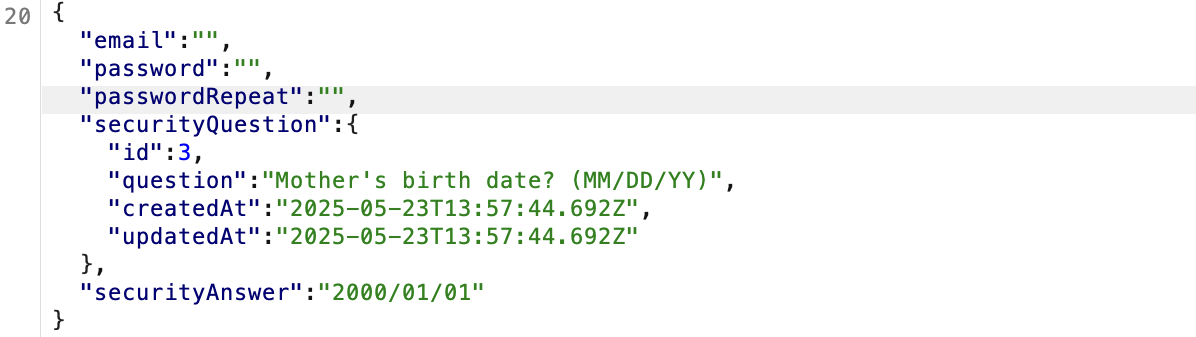
\includegraphics[width=0.7\textwidth]{empty-user.png}
    \caption{Use Burp to intercept the request}
    \label{fig:empty_user_registration}
  \end{figure}
\end{enumerate}

\subsection*{Login Bender $\bigstar\bigstar\bigstar$}
\textit{Steps:}
\begin{enumerate}
  \item Visit Juice Shop product lists, and view every product's comment to find bender's email. 
  \item I found out that bender's email is \texttt{bender@juice-sh.op}, at "Banana Juice (1000ml)"
  \item Login with bender's email and use SQL injection to bypass the password:
  \begin{itemize}
    \item email: \texttt{bender@juice-sh.op' --}
    \item password: \texttt{123456}
  \end{itemize}
\end{enumerate}

\subsection*{Login Jim $\bigstar\bigstar\bigstar$}
\textit{Steps:}
\begin{enumerate}
  \item Using the same method as "Login Bender", I found out that Jim's email is \texttt{jim@juice-sh.op}, at "Green Smoothie".
  \item Login with Jim's email and use SQL injection to bypass the password:
  \begin{itemize}
    \item email: \texttt{jim@juice-sh.op' --}
    \item password: \texttt{123456}
  \end{itemize}
\end{enumerate}

\subsection*{Forged Review $\bigstar\bigstar\bigstar$}
\textit{Steps:}
\begin{enumerate}
  \item After logined as jim, I visit the product list page and click one of the product to leave a review.
  \item I use burp to intercept the submin request. I changed the \texttt{author} field from \texttt{jim@juice-sh.op} to \texttt{bender@juice-sh.op}.
  \item After I forward the request, the task is completed.
\end{enumerate}

\subsection*{Error Handling $\bigstar$}
\textit{Steps:}
\begin{enumerate}
  \item I typed \texttt{jim', 1 or 1; --} in the login email field, and create an error.
\end{enumerate}

\subsection*{Upload Type $\bigstar\bigstar\bigstar$}
\textit{Steps:}
\begin{enumerate}
  \item I go to the \texttt{/ftp/quarantine} page and download the \texttt{juicy\_malware\_macos\_64.url} file.
  \item Visit the complain page.
  \item Select invoice file. I have to click "view options" in MacOS finder dialog box and change the format to \texttt{All Files} to upload the file. After that, I upload the "juicy malware" file.
\end{enumerate}

\section{Scoreboard}

% -----------------------------------------------------------
%    You don't have to mess with anything below this line.
% -----------------------------------------------------------

\end{document}
